% !TEX program = xelatex
\documentclass[11pt]{article}
\usepackage[margin=1in]{geometry}
\usepackage{nopageno} % no page numbers
\usepackage{setspace}

\usepackage{graphicx}
\graphicspath{ {./graphics/} }
\usepackage[dvipsnames]{xcolor}
\definecolor{CrispBlue}{HTML}{0176AE}

\usepackage{fontspec}
\usepackage{tcolorbox}
\usepackage{etoolbox}
\BeforeBeginEnvironment{verbatim*}{\begin{tcolorbox}[colback=CrispBlue!5!white,colframe=CrispBlue!75!black]}%
\AfterEndEnvironment{verbatim*}{\end{tcolorbox}}%

\usepackage{hyperref}
\hypersetup{
    colorlinks,
    citecolor=black,
    filecolor=black,
    linkcolor=black,
    urlcolor=black
}

\usepackage{subcaption}
\setlength{\parindent}{0pt}
\setlength{\parskip}{1em}

\usepackage{tocloft}
\renewcommand{\cftpartleader}{\cftdotfill{\cftdotsep}}
\renewcommand{\cftsecleader}{\cftdotfill{\cftdotsep}}

\usepackage[shortlabels]{enumitem}

\usepackage{fancyhdr}
\pagestyle{fancy}
\fancyhf{}
\lhead{ECE 517: Machine Learning}
\rhead{Assignment 6.3}
\rfoot{Page \thepage}

\usepackage{amsmath,amsfonts,amssymb}
\usepackage{bm}
\usepackage{mathtools}

\renewcommand{\listfigurename}{List of Figures}

\begin{document}
\setmainfont{SF Pro Text}
\setsansfont{SF Pro Text}
\setmonofont{SF Mono}
\renewcommand{\familydefault}{\sfdefault}

\thispagestyle{empty}
\begin{titlepage}
\vspace*{\fill}
\begin{center}
\textsc{\Huge{ECE 517: Machine Learning}}\\[3em]
\textsc{\LARGE Assignment 6.3: Nonlinear SVM Classifier}\\[6em]
\textsc{\Large David Kirby -- 101652098 -- davidkirby@unm.edu}\\[3em]
\textsc{\Large Fall 2021}
\end{center}
\vfill
\begin{figure}[h]
\begin{subfigure}{0.5\textwidth}

\includegraphics[width=0.25\linewidth]{learning.png}
\end{subfigure}
\begin{subfigure}{0.6\textwidth}\hspace{1em}

\includegraphics[width=0.8\linewidth]{new-soe-logo.png}
\end{subfigure}
\end{figure}
\end{titlepage}
\setcounter{figure}{0}

\hypersetup{
    linkcolor=CrispBlue,
    urlcolor=CrispBlue,
    breaklinks=true
}

\textbf{NONLINEAR SVM CLASSIFIER}

Use an SVM classifier to solve the classification problem of assignment 6.1.

\begin{enumerate}[A.]
    \item How to use the \texttt{svmtrain} function:\\If you type \texttt{svmtrain} you will see that the option \texttt{-t 4} exists, which allows the user to compute a kernel matrix and use it as an input instead of introducing the data. We will use this option to precompute the kernel matrix and place it in the position ``training\_instance\_matrix''. A similar option is present in Python.
    \item Work out a MATLAB or Python function whose input is the data matrix \( \mathbf{X} \) and whose output is the matrix of kernel dot products for:
    \begin{enumerate}[1.]
        \item Linear kernel.
        \item Order 3 polynomial kernel.
        \item Square exponential (also called Gaussian or Radial Basis Function) kernel with variable parameter \(\sigma\).
    \end{enumerate}
    \begin{itemize}
        \item Construct a training set of 100 samples and train a Support Vector Machine.
        \item Validate the parameter of the square exponential kernel and \(C\) with a validation set of 110 samples.
        \item Construct a test set of 1000 samples.
        \item Compute the kernel matrix between training and test sets. Compute the test error.
    \end{itemize}
    Do it for all three kernels.\\[1em]
    Provide the following:
    \begin{itemize}
        \item A draw of the classification boundary for the best values of validation parameters.
        \item Comments on the results.
    \end{itemize}
\end{enumerate}

\begin{tcolorbox}[colback=CrispBlue!5!white,colframe=CrispBlue!75!black,title=Nonlinear SVM Classifier.]\setstretch{1.25}
\texttt{LIBSVM} allows us to pass not only data through the support vector machine classifieer, but also kernel matrices. Using the kernel matrix function developed by the professor and his colleagues, we are able to create three classification boundaries -- linear, polynomial, and radial basis function.\\

Notice that the linear kernel does a fair job of classifying our data with about 10\% error. The polynomial kernel classifies the data very well, but tends to overfit the data. Finally, the RBF kernel classifies the data perfectly, with 0\% error and also solves the issue of overfitting.

\end{tcolorbox}

\begin{figure}[h!]
    \centering
    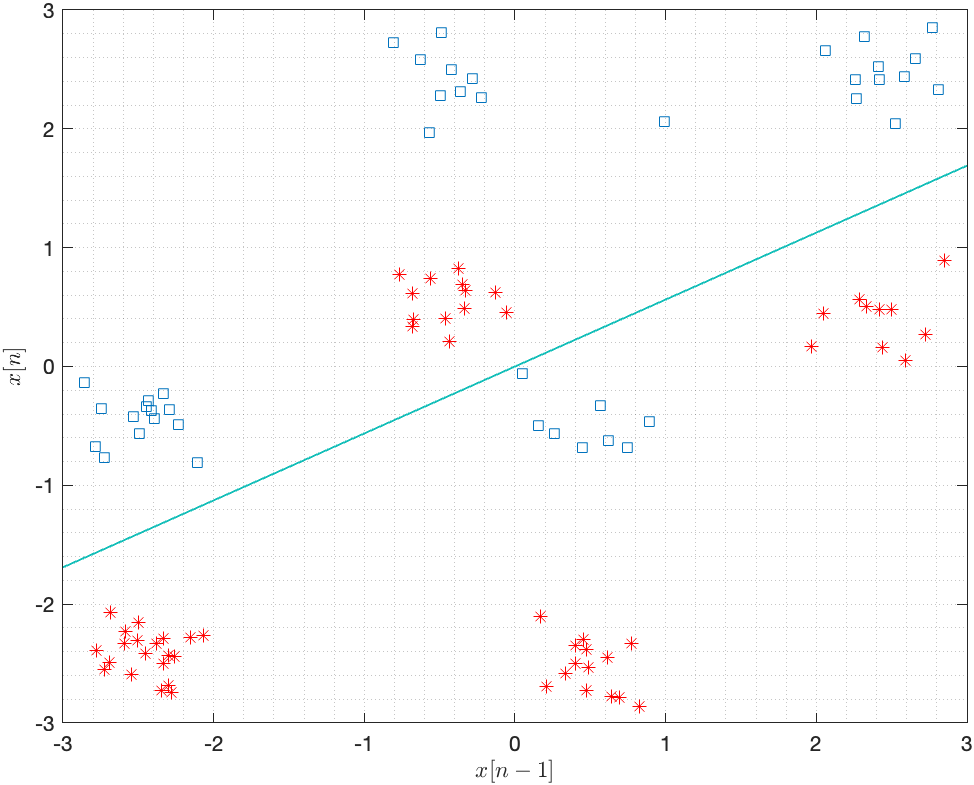
\includegraphics[width=\textwidth]{figure01.png}
    \caption{Linear kernel output.}
    \label{fig:linear}
\end{figure}

\begin{figure}[h!]
    \centering
    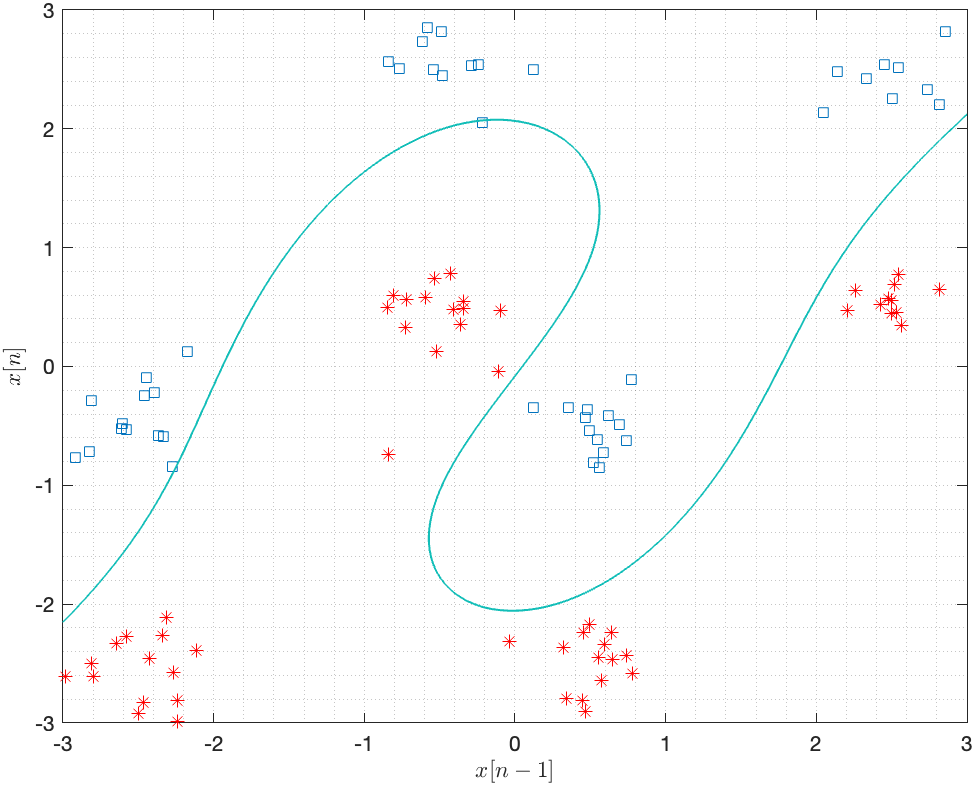
\includegraphics[width=\textwidth]{figure02.2.png}
    \caption{Polynomial kernel output.}
    \label{fig:poly}
\end{figure}

\begin{figure}[h!]
    \centering
    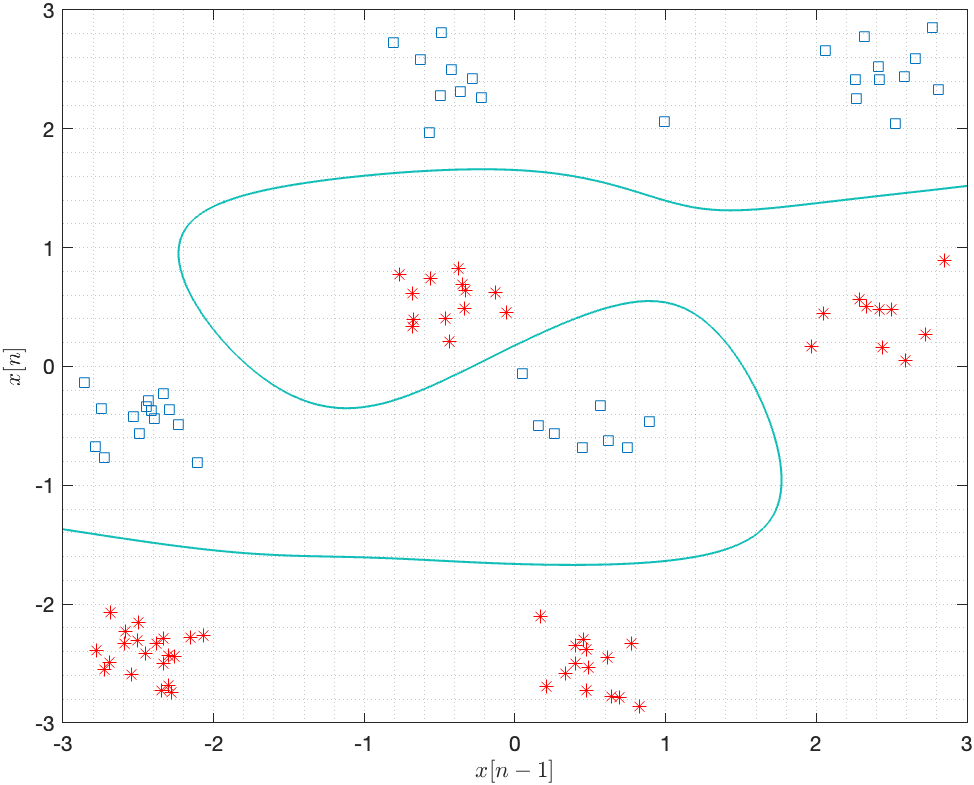
\includegraphics[width=\textwidth]{figure03.png}
    \caption{RBF kernel output.}
    \label{fig:rbf}
\end{figure}

\end{document}